\section{Electric Elements}
\kw{electric} elements are those elements that model electric and electronic
devices, dealing with abstract degrees of freedom more than with electric
ones (from the program's point of view they are exactly the same, the
difference is only semantic). The true electric elements, such resistors,
switches and so on, are classified as \kw{electric bulk} elements.
The syntax for \kw{electric} elements is:
%\begin{verbatim}
\begin{Verbatim}[commandchars=\\\{\}]
    \bnt{normal_arglist} ::= \bnt{electric_type} , \bnt{electric_arglist}
\end{Verbatim}
%\end{verbatim}
The \kw{electric} elements implemented at present are:
\begin{itemize}
	\item \kw{accelerometer}
	\item \kw{displacement}
	\item \kw{motor}
	\item \kw{discrete control}
\end{itemize}
The syntax is described in the following.

\subsection{Accelerometer}
%\begin{verbatim}
\begin{Verbatim}[commandchars=\\\{\}]
    \bnt{electric_type} ::= \kw{accelerometer}

    \bnt{electric_arglist} ::=
        \{ \kw{translational} | \kw{rotational} \} ,
        \bnt{struct_node_label} ,
        \bnt{abstract_node_label} ,
        ((\ty{Unit})\hty{Vec3}) \bnt{measure_direction}
        [ , \kw{position} , (\hty{Vec3}) \bnt{position} ]
\end{Verbatim}
%\end{verbatim}
The \kw{position} is optional; it is meaningless for \kw{rotational}
accelerometers.
The measure is taken along or about direction \nt{measure\_direction};
the vector is internally normalized to unity.

\noindent
Legacy element: accelerometer with built-in transfer function
%\begin{verbatim}
\begin{Verbatim}[commandchars=\\\{\}]
    \bnt{electric_type} ::= \kw{accelerometer}

    \bnt{electric_arglist} ::= \bnt{struct_node_label} ,
        \bnt{abstract_node_label} ,
        ((\ty{Unit})\hty{Vec3}) \bnt{measure_direction} ,
        (\ty{real}) \bnt{omega} ,
        (\ty{real}) \bnt{tau} ,
        (\ty{real}) \bnt{csi} ,
        (\ty{real}) \bnt{kappa}	
\end{Verbatim}
%\end{verbatim}
The label \nt{struct\_node\_label} defines the node whose acceleration 
is being measured; the label \nt{abstract\_node\_label} defines the
\kw{abstract node} that will receive the output signal. 
An \kw{electric node} can be used as well (?).
The measure is taken along direction \nt{measure\_direction};
the vector is internally normalized to unity.
The transfer function of the accelerometer is:
\begin{displaymath}
    \frac{e_0}{a} = \nt{kappa} \cdot \frac{\nt{tau} \cdot s}{
        \plbr{1 + \nt{tau} \cdot s}
        \plbr{1 + 2 \cdot \nt{csi} \cdot (s/\nt{omega}) + (s/\nt{omega})^2}
    }
\end{displaymath}
where $ e_0 $ is the output signal, $ a $ is the input (the acceleration)
and $ s $ is Laplace's variable.



\subsection{Discrete control}\label{sec:EL:DISCCTRL}
This element implements a discrete equation
that can be used to represent the behavior
of a discrete linear controller.
The control matrices can be either provided,
or identified during the simulation by recursive least squares.

Assume the original system consists in a generic nonlinear process
that depends on a set of measures $\T{y}$ and a set of inputs $\T{u}$
at a finite number of time steps past the current time, $t_k$, namely
\begin{align}
	\T{f}\plbr{\T{y}_{k - i}, \T{u}_{k - j}} = \T{0} ,
\end{align}
with $i=0,p$ and $j=0,q$.
Only $\T{y}_k$ is unknown, and thus represents the output of the process.
It is assumed that $\T{u}_k$ is known, and represents an input
to the process.

This element implements a controller of the form
\begin{align}
	\T{u}_{ck}
	&= \sum_{i=1,p} \TT{B}_{ci} \T{u}_{k - i}
	+ \sum_{j=1,q} \TT{A}_{cj} \T{y}_{k - j} ,
\end{align}
where $\T{u}_{ck}$ is the control input that must be applied
at time $t_k$ in addition to any exogenous input $\T{u}_{ek}$,
so that $\T{u}_k = \T{u}_{ek} + \T{u}_{ck}$.
The control input $\T{u}_{ck}$ can only depend on the measures
and the inputs at previous time steps.

Note that the symbols commonly used for discrete systems
are here reversed, since the element is intended to compute
the control signals at time $t_k$, $\T{u}_{ck}$,
based on the previous value of the controls,
$\T{u}_{k-i} = \T{u}_{e(k - i)} + \T{u}_{c(k - i)}$,
and on the previous value of the motion of the original system,
$\T{y}_{k-j}$;
$\T{u}_e$ indicates a generic measured exogenous input
to the system to be controlled.

The order $p$ and $q$ of the auto-regressive and exogenous portions
of the system can differ.
In detail, the order $p$ can be zero; in that case, the system
implements a \emph{finite impulse response} function.

This element is not self-starting; it assumes that both
inputs and outputs at times before the start time are zero.

The so-called ``output'' signals, indicated with $\T{y}$,
can be instances of either \hty{NodeDof} or \hty{DriveCaller} objects.
The so-called ``input'' signals, indicated with $\T{u}$,
must be instances of \hty{NodeDof} object.
This implies that instances of \hty{NodeDof} objects
need the corresponding equations to be (at least) statically defined.
In fact, the \kw{discrete control} element uses the ``output''
\hty{NodeDof} values, the $\T{y}$, to compute the corresponding
``inputs'', the $\T{u}$.
The latter are substantially added as a right-hand side
to the equations of the corresponding \hty{NodeDof} objects.
As a consequence, other elements must contribute to the left-hand side
of all the \hty{NodeDof} equations in order to make them defined.

Note that other elements may also contribute to the right-hand side
of the ``input'' \hty{NodeDof} object.
Specifically, other \kw{abstract} forces may contribute to their value.
In that case, the additional forces represent the exogenous inputs.
They are considered as part of the input used by the \kw{discrete control}
element, since the value $\T{u}_k$ to be used in the control equation
is extracted from the value of the corresponding \hty{NodeDof} objects.

Figure~\ref{fig:discctrl} illustrates the behavior of the element.
The typical suggested approach is illustrated later in an example.
\begin{figure}
\centering
\psfrag{A}{$\TT{A}$}
\psfrag{B}{$\TT{B}$}
\psfrag{f}{$\T{f}$}
\psfrag{uc}{$\T{u}_c$}
\psfrag{fe}{$\T{u}_e$}
\psfrag{uk-2}{$\T{u}_{k-2}$}
\psfrag{uk-1}{$\T{u}_{k-1}$}
\psfrag{uk}{$\T{u}_{k}$}
\psfrag{yk-2}{$\T{y}_{k-2}$}
\psfrag{yk-1}{$\T{y}_{k-1}$}
\psfrag{yk}{$\T{y}_{k}$}
\psfrag{k=1}{$\mathbb{K}=1$}
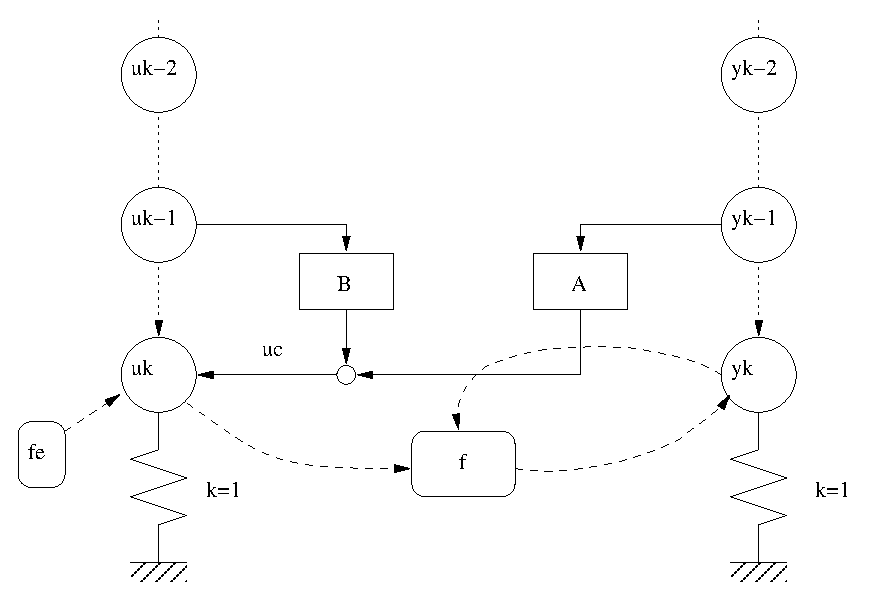
\includegraphics[width=.7\textwidth]{discctrl}
\caption{Discrete control layout.}
\label{fig:discctrl}
\end{figure}

The syntax is
%\begin{verbatim}
\begin{Verbatim}[commandchars=\\\{\}]
    \bnt{electric_type} ::= \kw{discrete control}

    \bnt{electric_arglist} ::= \bnt{num_outputs} , \bnt{num_inputs} ,
        \bnt{order_A} [ , \kw{fir} , \bnt{order_B} ] ,
        \bnt{num_iter} ,
        \bnt{control_data} , 
        \kw{outputs} ,
            (\ty{ScalarValue}) \bnt{output_value}
                [ , \kw{scale} , (\hty{DriveCaller}) \bnt{scale} ]
            [ , ... ] ,
        \kw{inputs} ,
            (\hty{NodeDof}) \bnt{input_dof}
            [ , ... ]

    \bnt{output_value} ::=
        \{ [ \kw{node dof} , ] (\hty{NodeDof}) \bnt{output_dof}
            | \kw{drive} , (\hty{DriveCaller}) \bnt{output_drive} \}
\end{Verbatim}
%\end{verbatim}
The lists of the output and input dofs follows. The inputs
do not require the \nt{order\_A} and \nt{order\_B} fields,
since they are simply used to compute the control forces,
and thus identify an equation.
\nt{order\_B} defaults to \nt{order\_A} unless a \kw{fir} control is chosen.

The \nt{control\_data} has the syntax:
%\begin{verbatim}  
\begin{Verbatim}[commandchars=\\\{\}]
        \bnt{control_data} ::= \bnt{control_type} , \bnt{control_arglist}
\end{Verbatim}
%\end{verbatim}
At present only a simple form of control is implemented. Other types
to come are system identification, both recursive and one-shot, and
adaptive control, with different models and schemes, all based on 
Generalized Predictive Control (GPC) and Deadbeat Control.
The \nt{control\_data} syntax is:
%\begin{verbatim}
\begin{Verbatim}[commandchars=\\\{\}]
    \bnt{control_data} ::=
        \{ \kw{control} , " \bnt{control_matrices_file} "
            | \kw{identification} , \bnt{identification_data}
            | \kw{adaptive control} , \bnt{adaptive_control_data} \}
\end{Verbatim}
%\end{verbatim}

\subsubsection{Control}
The file \nt{control\_matrices\_file} must contain the matrices
$ a_c $, $ b_c $ of the control in plain text (as generated by Matlab, for
instance):

\noindent
\begin{tabular}{l}
    $ a_{c1} $, \\
    \ldots,     \\
    $ a_{cp} $, \\
    $ b_{c1} $, \\
    \ldots,     \\
    $ b_{cp} $  \\
\end{tabular} \\
where $ p $ is the \nt{order\_A} of the controller and the matrices $ a_c $
have \nt{num\_inputs} rows and \nt{num\_outputs} columns, while the
matrices $ b_c $ have \nt{num\_inputs} rows and \nt{num\_inputs} columns.

\subsubsection{Identification}
%\begin{verbatim}
\begin{Verbatim}[commandchars=\\\{\}]
    \bnt{identification_data} ::=
        \{ \kw{arx} | \kw{armax} \}
        [ , \bnt{forgetting_factor} ]
        [ , \bnt{persistent_excitation} ]
        [ , \kw{file} , " \bnt{output_file_name} " ]
\end{Verbatim}
%\end{verbatim}
The forgetting factor is defined as
%\begin{verbatim}
\begin{Verbatim}[commandchars=\\\{\}]
    \bnt{forgetting_factor} ::=
        \kw{forgettingfactor} ,
          \{ \kw{const} , \bnt{d}
              | \kw{dynamic} , \bnt{n1} , \bnt{n2} , \bnt{rho} , \bnt{fact} , \bnt{kref} , \bnt{klim} \}
\end{Verbatim}
%\end{verbatim}
The default is a \kw{const} forgetting factor with $\nt{d}=1$.

The \nt{persistent\_excitation} is defined as
%\begin{verbatim}
\begin{Verbatim}[commandchars=\\\{\}]
    \bnt{persistent_excitation} ::=
        \kw{excitation} , (\hty{DriveCaller}) \bnt{excitation_drive} [ , ... ]
\end{Verbatim}
%\end{verbatim}
where \nt{num\_inputs} instances of \nt{excitation\_drive} must be defined.
By default, no persistent excitation is defined.

\subsubsection{Adaptive control}
The \nt{adaptive\_control\_data} card is
%\begin{verbatim}
\begin{Verbatim}[commandchars=\\\{\}]
    \bnt{adaptive_control_data} ::=
        [ \{ \kw{arx} | \kw{armax} \} , ]
        [ \kw{periodic} , \bnt{periodic_factor} , ]
        \{ \kw{gpc} ,
            \bnt{prediction_advancing_horizon} ,
            \bnt{control_advancing_horizon} ,
            \bnt{prediction_receding_horizon} ,
            [ \kw{prediction weights} , \bnt{Wi} [ , ... ] , ]
            [ \kw{control weights} , \bnt{Ri} [ , ... ] , ]
            (\hty{DriveCaller}) \bnt{weight_drive}
        | \kw{deadbeat} ,
            \bnt{prediction_advancing_horizon} ,
            \bnt{control_advancing_horizon} \}
        [ , \bnt{forgetting_factor} ]
        [ , \bnt{persistent_excitation} ]
        [ , \kw{trigger} , (\hty{DriveCaller}) \bnt{trigger_drive} ]
        [ , \kw{desired output} , (\hty{DriveCaller}) \bnt{output_drive} [ , ... ] ]
        [ , \kw{file} , " \bnt{file_name} " ]
\end{Verbatim}
%\end{verbatim}
The default is \kw{arx}.

The meaning of the keywords is:
\begin{itemize}
\item the \nt{periodic\_factor} defaults to 0;

\item if the keyword \kw{prediction weights} is present,
a number of weights \nt{Wi} equal to
\begin{quote}
$(\nt{prediction\_advancing\_horizon} - \nt{prediction\_receding\_horizon})$
\end{quote}
must be supplied.
If the keyword \kw{control weights} is present,
a number of weights \nt{Ri} equal to \nt{control\_advancing\_horizon}
must be supplied.
If the keywords are not defined, the corresponding weights
default to 1;

\item the \kw{desired output}
option requires \nt{num\_outputs} drives to be defined.
\end{itemize}

\subsubsection{Private Data}
The following data are available:
\begin{enumerate}
\item \kw{"u[\bnt{idx}]"} value of the \nt{idx}-th control output.
\end{enumerate}

\subsubsection{Examples}
Consider the case of a discrete controller that computes
a set of control signals $\T{u}_k$ by adding to their value
at the previous step, $\T{u}_{k-1}$, a contribution coming
from some measure $\T{y}_{k-1}$.
The control matrices are
\begin{subequations}
\begin{align}
	\TT{A}_{c1}
	&=
	\sqbr{\matr{cc}{
		a_{11} & a_{12} \\
		a_{21} & a_{22}
	}}
	\\
	\TT{B}_{c1}
	&=
	\sqbr{\matr{cc}{
		1 & 0 \\
		0 & 1
	}}
\end{align}
\end{subequations}
They are defined in the control data file \texttt{discretecontrol.dat} as
\begin{verbatim}
    a_11 a_12
    a_21 a_22
    1.0 0.0
    0.0 1.0
\end{verbatim}
The model consists in two abstract nodes for the control input
\hty{NodeDof} objects.
They need to be grounded.
This can be formulated by using a \kw{spring support} \kw{genel}
for each \kw{abstract} node, characterized by a unit spring coefficient,
such that
\begin{subequations}
\begin{align}
	1 \cdot x_{u1} &= u_1
	\\
	1 \cdot x_{u2} &= u_2
\end{align}
\end{subequations}
Moreover, assume that the first measure, $y_1$,
comes from a \hty{NodeDof} object,
while the second one, $y_2$, comes from a \hty{DriveCaller} object.
The equation corresponding to $y_1$ must be appropriately grounded
as well, for example by means of yet another \kw{spring support}
\kw{genel}.
This is outside the scope of the present example, so it will assume
the output nodes are defined appropriately.

The model is
\begin{verbatim}
    set: integer U_1 = 1;
    set: integer U_2 = 2;
    set: integer Y_1 = 11;
    # ...
    abstract: U_1;
    abstract: U_2;
    # ...
    genel: U_1, spring support,
        U_1, abstract, algebraic,
        linear elastic, 1.;
    genel: U_2, spring support,
        U_2, abstract, algebraic,
        linear elastic, 1.;
    electric: 99, discrete control,
        2,    # number of `outputs' y
        2,    # number of `inputs' u
        1,    # order of output matrices A (same for input matrices B)
        1,    # update every iteration
        control, "discretecontrol.dat",
        outputs,
            node dof, Y_1, abstract, algebraic, scale, 1.e-3,
            drive, sine, .5, 2*pi, 1., forever, 0, scale, 1.e-3,
        inputs,
            U_1, abstract, algebraic,
            U_2, abstract, algebraic;
\end{verbatim}



\subsection{Displacement}
%\begin{verbatim}
\begin{Verbatim}[commandchars=\\\{\}]
    \bnt{electric_type} ::= \kw{displacement}

    \bnt{electric_arglist} ::=
        \bnt{struct_node_1_label} , (\hty{Vec3}) \bnt{relative_offset_1} ,
        \bnt{struct_node_2_label} , (\hty{Vec3}) \bnt{relative_offset_2} ,
        \bnt{abstract_node_label}
\end{Verbatim}
%\end{verbatim}
\begin{subequations}
\begin{align}
	\T{d} &= \T{x}_b + \T{o}_b - \T{x}_a - \T{o}_a \\
	x &= \sqrt{\T{d}^T \T{d}}
\end{align}
\end{subequations}
The value $x$ is added to the right-hand side of the equation
of the \kw{abstract} node.

\subsection{Motor}
%\begin{verbatim}
\begin{Verbatim}[commandchars=\\\{\}]
    \bnt{electric_type} ::= \kw{motor}

    \bnt{electric_arglist} ::=
        \bnt{struct_node_1_label} ,
        \bnt{struct_node_2_label} ,
        ((\ty{Unit})\hty{Vec3}) \bnt{direction_relative_to_node_1} ,
        \bnt{abstract_node_1_label} ,
        \bnt{abstract_node_2_label} ,
        (\ty{real}) \bnt{dG},
        (\ty{real}) \bnt{dL},
        (\ty{real}) \bnt{dR}
        [ , \kw{initial current} , \bnt{i_0} ]
\end{Verbatim}
%\end{verbatim}
This element implements a simple DC motor, whose equations are
\begin{subequations}
\begin{align}
	\omega &= \T{e}^T \plbr{\T{\omega}_2 - \T{\omega}_1} \\
	V &= V_2 - V_1 \\
	V &= \nt{dL} \frac{\mathrm{d}i}{\mathrm{d}t} + \nt{dR} \, i + \nt{dG} \, \omega \\
	\T{c}_1 &= - \T{e} \, \nt{dG} \, i \\
	\T{c}_2 &= \T{e} \, \nt{dG} \, i \\
	i_1 &= -i \\
	i_2 &= i
\end{align}
\end{subequations}
where \nt{dL} is the inductance, \nt{dR} is the resistance, and \nt{dG} is the motor torque/back-EMF constant.

The motor applies an internal torque, $C = \nt{dG} \, i$, about direction
$\T{e}=\nt{direction\_relative\_to\_node\_1}$, with opposite sign
to both the structural nodes it is connected to, namely \nt{struct\_node\_1\_label} and \nt{struct\_node\_2\_label}.
The input vector that represents direction $\T{e}$ is internally normalized to unity.

It also contributes with a current $i$ to both the electrical nodes it is connected to,
the abstract nodes \nt{abstract\_node\_1\_label} and \nt{abstract\_node\_2\_label}.

The element assumes that the only allowed relative motion between nodes 1 and 2 is a rotation about direction $\T{e}$,
so appropriate joints (e.g.\ a \kw{total joint}, a \kw{revolute hinge}, or \kw{revolute pin}) must be in place.


